\PassOptionsToPackage{table}{xcolor}
\documentclass[10pt,aspectratio=169]{beamer}

% Presentación autocontenida para TeX Live y LaTeX Workshop.
% Compilación recomendada: latexmk -pdf presentacion_clinica_15min.tex
% Las notas del expositor se conservan en el código mediante \note{...}.

\usepackage[utf8]{inputenc}
\usepackage[T1]{fontenc}
\usepackage[spanish,es-nodecimaldot]{babel}
\usepackage{lmodern}
\usepackage{microtype}
\usepackage{graphicx}
\usepackage{booktabs}
\usepackage{tabularx}
\usepackage{array}
\usepackage{tikz}
\usetikzlibrary{arrows.meta,positioning,calc}
\usepackage{ragged2e}

\definecolor{AzulClinica}{HTML}{0F3D5E}
\definecolor{AzulTecnologia}{HTML}{247BA0}
\definecolor{Turquesa}{HTML}{16A6A1}
\definecolor{FondoClaro}{HTML}{F4F8FA}
\definecolor{GrisTexto}{HTML}{475569}
\definecolor{Borde}{HTML}{D8E4EA}
\definecolor{VerdeClaro}{HTML}{DDF5F2}
\definecolor{AzulClaro}{HTML}{E2F0F7}
\definecolor{NaranjaSuave}{HTML}{F59E0B}

\usetheme{default}
\setbeamertemplate{navigation symbols}{}
\setbeamercolor{normal text}{fg=AzulClinica,bg=white}
\setbeamercolor{frametitle}{fg=AzulClinica,bg=white}
\setbeamercolor{structure}{fg=Turquesa}
\setbeamercolor{itemize item}{fg=Turquesa}
\setbeamercolor{itemize subitem}{fg=AzulTecnologia}
\setbeamerfont{frametitle}{size=\Large,series=\bfseries}
\setbeamerfont{title}{size=\huge,series=\bfseries}
\setbeamerfont{subtitle}{size=\large}
\setbeamersize{text margin left=8mm,text margin right=8mm}

\newcommand{\expositor}{Equipo completo}
\newcommand{\tiempo}{15:00}
\newcommand{\presenta}[2]{\gdef\expositor{#1}\gdef\tiempo{#2}}
\newcommand{\destacado}[1]{\textcolor{Turquesa}{\textbf{#1}}}
\newcommand{\servicio}[1]{\textcolor{AzulTecnologia}{\textbf{#1}}}
\newcommand{\fuente}[1]{\vspace{0.15cm}{\scriptsize\color{GrisTexto}#1}}

\setbeamertemplate{frametitle}{%
  \vspace{0.35cm}\insertframetitle\par
  \vspace{-0.12cm}\textcolor{Turquesa}{\rule{1.25cm}{1.6pt}}
}

\setbeamertemplate{footline}{%
  \leavevmode
  \hbox{%
    \begin{beamercolorbox}[wd=.76\paperwidth,ht=3.2ex,dp=1.35ex,leftskip=8mm]{normal text}%
      \tiny\color{GrisTexto}Expone: \textbf{\expositor}\hspace{1.2em}
    \end{beamercolorbox}%
    \begin{beamercolorbox}[wd=.24\paperwidth,ht=3.2ex,dp=1.35ex,rightskip=8mm plus 1fil]{normal text}%
      \hfill\tiny\color{GrisTexto}Clínica del Sur\hspace{1em}\insertframenumber/\inserttotalframenumber
    \end{beamercolorbox}%
  }
}

\setbeamertemplate{itemize item}{\raise0.15ex\hbox{\color{Turquesa}\small$\blacktriangleright$}}
\setbeamertemplate{itemize subitem}{\raise0.12ex\hbox{\color{AzulTecnologia}\tiny$\bullet$}}
\setlength{\leftmargini}{1.25em}
\setlength{\leftmarginii}{1.05em}

\newcolumntype{Y}{>{\RaggedRight\arraybackslash}X}
\newcolumntype{C}[1]{>{\Centering\arraybackslash}p{#1}}

\title{Clínica del Sur}
\subtitle{Arquitectura de datos en AWS para una gestión clínica basada en información}
\author{Genesis Callisaya \and Cristhian Rodrigo Alave Sanjines \and Samuel Loza Ramirez \and Liceth Quispe Apaza}
\institute{Universidad Mayor de San Andrés\\Postgrado en Informática · Módulo V}
\date{La Paz, Bolivia · 1 de octubre de 2026}

\begin{document}

\presenta{Equipo completo}{0:40}
\begin{frame}[plain]
  \begin{tikzpicture}[remember picture,overlay]
    \fill[FondoClaro] (current page.south west) rectangle (current page.north east);
    \fill[AzulClinica] (current page.south west) rectangle ([xshift=4.25cm]current page.north west);
    \fill[Turquesa] ([xshift=4.05cm]current page.south west) rectangle ([xshift=4.25cm]current page.north west);
    \node[anchor=north west] at ([xshift=0.65cm,yshift=-0.65cm]current page.north west)
      {
\includegraphics[width=2.95cm]{figures/logo_postgrado.png}};
    \node[anchor=south west,text width=3.0cm,align=left,text=white] at ([xshift=0.65cm,yshift=0.72cm]current page.south west)
      {\scriptsize Universidad Mayor de\\San Andrés\\[0.15cm]Postgrado en Informática\\Módulo V};
  \end{tikzpicture}
  \hspace*{4.25cm}
  \begin{minipage}[c][0.79\textheight][c]{0.64\textwidth}
    {\color{Turquesa}\bfseries PROPUESTA ACADÉMICA}\par\vspace{0.22cm}
    {\fontsize{31}{34}\selectfont\bfseries\color{AzulClinica}Clínica del Sur}\par\vspace{0.25cm}
    {\Large\color{GrisTexto}\RaggedRight Arquitectura de datos en AWS para una\\gestión clínica basada en información}\par
    \vspace{0.55cm}
    {\small\color{AzulClinica}\textbf{Equipo expositor}}\par
    {\small Genesis Callisaya · Cristhian Rodrigo Alave Sanjines}\par
    {\small Samuel Loza Ramirez · Liceth Quispe Apaza}\par
    \vspace{0.35cm}
    {\scriptsize\color{GrisTexto}La Paz, Bolivia · 1 de octubre de 2026}
  \end{minipage}
  \note{Genesis abre la exposición. Presentar el caso como una propuesta académica para una clínica ficticia. Indicar que el trabajo conecta el problema de negocio con un modelo relacional, almacenamiento documental, control de acceso, indicadores y metas. Aclarar desde el inicio que no se mostrarán datos clínicos reales ni se afirmará que existen recursos desplegados en AWS. Nombrar al equipo y anticipar el reparto: Genesis explicará el contexto y cerrará; Samuel desarrollará los datos y RDS; Cristhian presentará S3, IAM y la arquitectura; Liceth explicará los KPI y el OKR. La exposición está organizada para durar aproximadamente quince minutos.}
\end{frame}

\presenta{Genesis Callisaya}{1:20}
\begin{frame}{Contexto y problema del negocio}
  \begin{columns}[T,onlytextwidth]
    \column{0.50\textwidth}
      {\Large\bfseries La clínica genera información todos los días}\par\vspace{0.25cm}
      \begin{itemize}
        \item Pacientes, médicos y especialidades.
        \item Consultorios, citas y atenciones.
        \item Consultas, pagos y documentos médicos.
      \end{itemize}
      \vspace{0.2cm}
      {\color{GrisTexto}Sin una estructura común, los registros quedan distribuidos en archivos o sistemas separados.}
    \column{0.46\textwidth}
      \begin{tikzpicture}[x=1cm,y=1cm]
        \node[draw=Borde,fill=FondoClaro,rounded corners=4pt,text width=5.0cm,minimum height=1.0cm,align=left] (a) at (0,2.45) {\textbf{Información distribuida}\\\small Dificulta obtener una visión actualizada.};
        \node[draw=Borde,fill=FondoClaro,rounded corners=4pt,text width=5.0cm,minimum height=1.0cm,align=left] (b) at (0,1.10) {\textbf{Gestión de citas}\\\small Cuesta seguir atenciones, cancelaciones y ausencias.};
        \node[draw=Borde,fill=FondoClaro,rounded corners=4pt,text width=5.0cm,minimum height=1.0cm,align=left] (c) at (0,-0.25) {\textbf{Decisiones con poca evidencia}\\\small La demanda y el uso de recursos no se observan con facilidad.};
        \draw[-{Latex},thick,Turquesa] (a) -- (b);
        \draw[-{Latex},thick,Turquesa] (b) -- (c);
      \end{tikzpicture}
  \end{columns}
  \note{Explicar que la Clínica del Sur atiende distintas especialidades y produce información operativa y clínica de manera continua. El problema principal no es la falta de datos, sino su dispersión. Cuando pacientes, citas y atenciones se registran en lugares diferentes, resulta difícil responder preguntas simples: cuántas personas fueron atendidas, qué especialidad tiene mayor demanda o qué proporción de citas terminó cancelada. Esta situación también complica el seguimiento de los recursos disponibles. La propuesta parte de esa necesidad y no de una tecnología elegida de antemano. La arquitectura se justifica porque organiza la información y permite consultarla de manera consistente. Transición: una vez entendido el problema, se define el objetivo estratégico y las preguntas que la solución debe contestar.}
\end{frame}

\presenta{Genesis Callisaya}{1:10}
\begin{frame}{Objetivo estratégico y necesidades de información}
  \begin{tikzpicture}[remember picture,overlay]
    \fill[AzulClaro] ([xshift=8mm,yshift=-18mm]current page.north west) rectangle ([xshift=-8mm,yshift=-42mm]current page.north east);
    \node[anchor=west,text width=13.2cm,align=left] at ([xshift=13mm,yshift=-30mm]current page.north west)
      {\large\bfseries\color{AzulClinica}Mejorar la gestión de las citas y la atención mediante el análisis de datos, para optimizar los servicios y el uso de los recursos disponibles.};
  \end{tikzpicture}
  \vspace{2.35cm}
  \begin{columns}[T,onlytextwidth]
    \column{0.31\textwidth}
      {\color{Turquesa}\Large\bfseries 01}\par
      \textbf{Demanda}\par
      ¿Qué especialidades concentran más atenciones?
    \column{0.31\textwidth}
      {\color{Turquesa}\Large\bfseries 02}\par
      \textbf{Cumplimiento}\par
      ¿Cuántas citas se atienden, cancelan o quedan sin atención?
    \column{0.31\textwidth}
      {\color{Turquesa}\Large\bfseries 03}\par
      \textbf{Capacidad}\par
      ¿Cómo distribuir médicos y consultorios según la actividad?
  \end{columns}
  \vfill
  \fuente{La arquitectura debe convertir estas preguntas en consultas repetibles y KPI verificables.}
  \note{Leer el objetivo estratégico de forma breve y explicar cómo se traduce en necesidades de información. La primera necesidad consiste en medir la demanda por especialidad para decidir dónde se requieren más médicos, horarios o consultorios. La segunda consiste en conocer el resultado de cada cita y detectar cancelaciones o inasistencias. La tercera relaciona esa demanda con la capacidad disponible. Destacar que estas preguntas orientan el modelo de datos. No conviene almacenar información sin saber para qué se utilizará. La propuesta sigue una secuencia clara: el negocio define preguntas; las tablas registran los hechos; AWS organiza y protege los datos; los KPI resumen la operación; el OKR fija metas. Transición al siguiente expositor: Samuel explicará qué datos necesita la clínica y cómo se organizan en Amazon RDS.}
\end{frame}

\presenta{Samuel Loza Ramirez}{1:40}
\begin{frame}{Datos estructurados en Amazon RDS}
  \begin{columns}[T,onlytextwidth]
    \column{0.58\textwidth}
      \begin{tikzpicture}[node distance=4mm and 5mm,
        entidad/.style={draw=Borde,fill=white,rounded corners=4pt,minimum width=3.1cm,minimum height=.88cm,align=center,font=\small\bfseries},
        flecha/.style={-{Latex[length=2mm]},thick,draw=Turquesa}]
        \node[entidad] (pac) {PACIENTE};
        \node[entidad,right=of pac] (esp) {ESPECIALIDAD};
        \node[entidad,below=of esp] (med) {MÉDICO};
        \node[entidad,below=of pac] (con) {CONSULTORIO};
        \node[entidad,below=of con,xshift=1.72cm] (cit) {CITA};
        \node[entidad,below=of cit] (ate) {ATENCIÓN};
        \draw[flecha] (esp) -- (med);
        \draw[flecha] (pac) -- (cit);
        \draw[flecha] (med) -- (cit);
        \draw[flecha] (con) -- (cit);
        \draw[flecha] (cit) -- (ate);
      \end{tikzpicture}
    \column{0.38\textwidth}
      {\Large\bfseries Función de RDS}\par\vspace{0.2cm}
      \begin{itemize}
        \item Conserva datos estructurados en MySQL.
        \item Aplica claves primarias, foráneas y restricciones.
        \item Permite consultas para los KPI.
        \item Separa la operación de los archivos clínicos.
      \end{itemize}
  \end{columns}
  \vfill
  \begin{tikzpicture}
    \node[fill=VerdeClaro,rounded corners=4pt,text width=13.7cm,align=center,inner sep=6pt] {\textbf{Regla principal:} una CITA vincula paciente, médico y consultorio; una ATENCIÓN documenta el resultado de esa cita.};
  \end{tikzpicture}
  \note{Samuel presenta las seis entidades del modelo base. PACIENTE identifica a la persona atendida. ESPECIALIDAD clasifica los servicios médicos. MÉDICO pertenece a una especialidad. CONSULTORIO representa el espacio asignable. CITA conecta paciente, médico, consultorio, fecha, hora y estado. ATENCIÓN registra el resultado asistencial y se relaciona de manera única con una cita. Las claves primarias identifican cada registro y las claves foráneas mantienen las relaciones. Amazon RDS con MySQL resulta adecuado para estos datos porque existe una estructura definida y necesitamos consultas consistentes. Señalar que RDS no guarda directamente archivos PDF o imágenes de estudios. También aclarar que el KPI mensual debe contar pacientes únicos cuando esa sea la definición, mediante la relación ATENCIÓN, CITA y PACIENTE. Transición: la siguiente diapositiva muestra el modelo completo y sus ampliaciones.}
\end{frame}

\presenta{Samuel Loza Ramirez}{1:30}
\begin{frame}{Modelo relacional: base y ampliaciones}
  \begin{columns}[c,onlytextwidth]
    \column{0.72\textwidth}
      \centering
      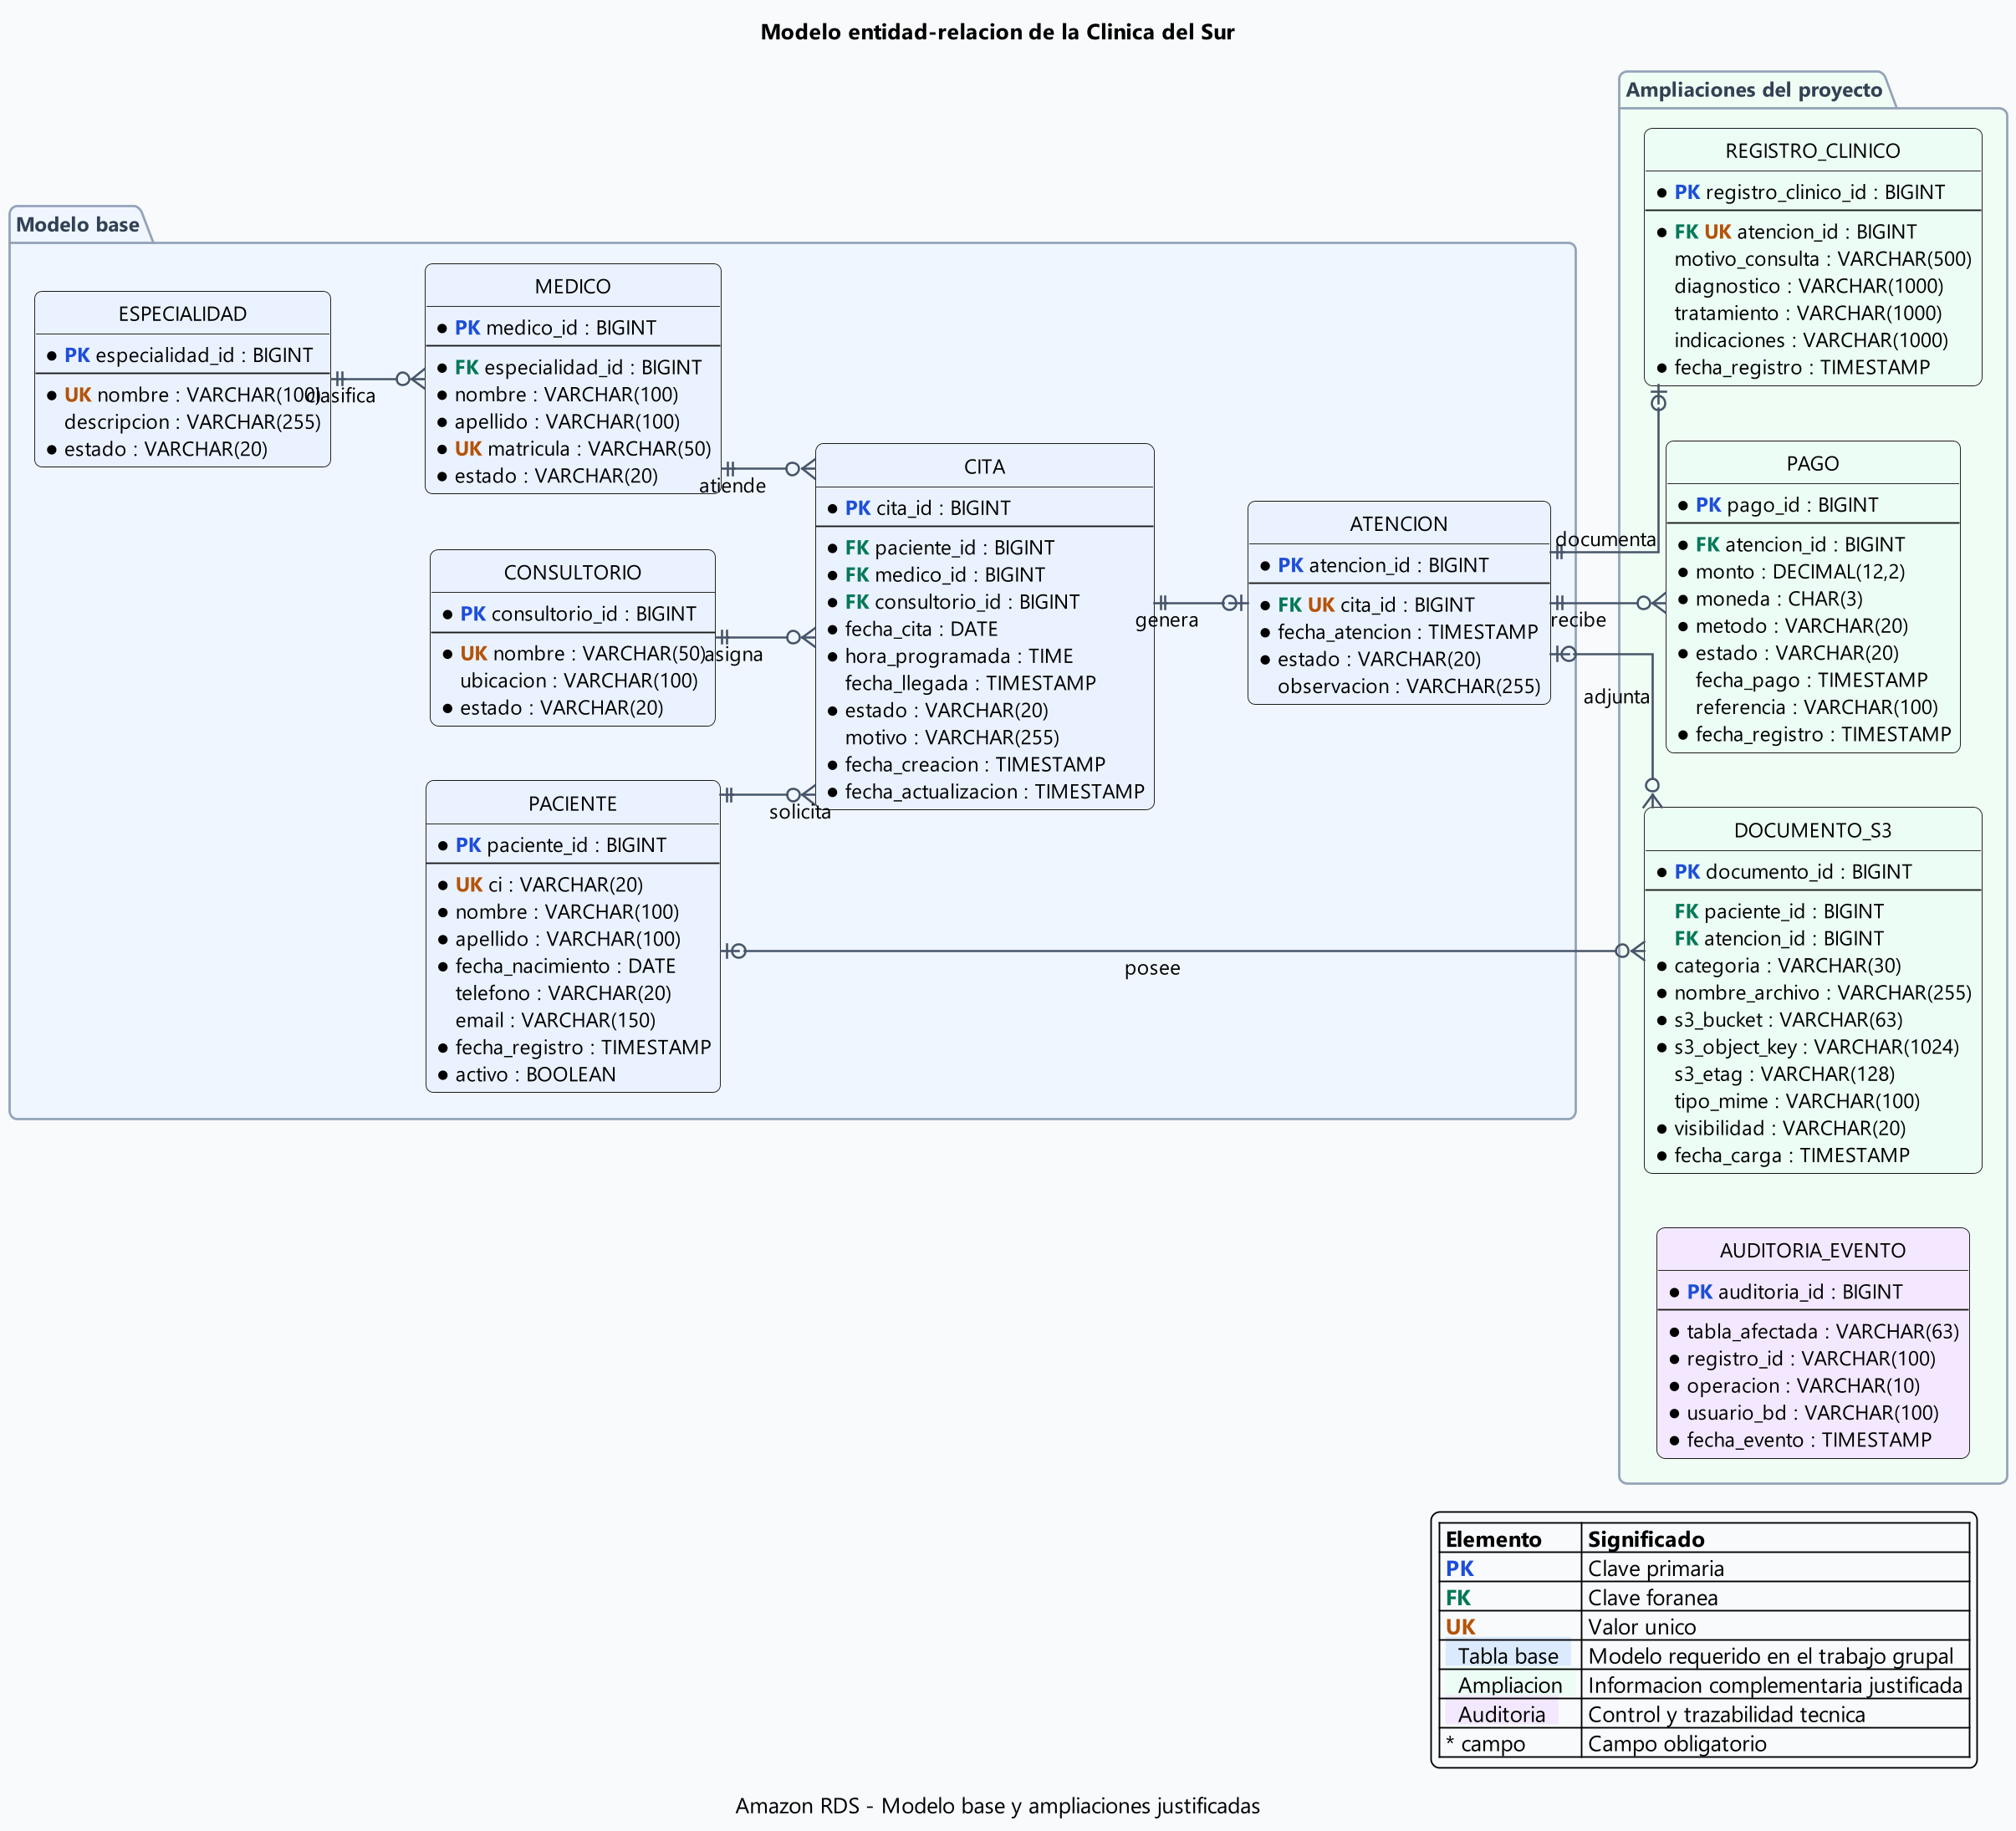
\includegraphics[width=\linewidth,height=0.69\textheight,keepaspectratio]{figures/modelo_datos_plantuml.png}
    \column{0.25\textwidth}
      {\color{AzulTecnologia}\bfseries MODELO BASE}\par
      {\small Paciente, especialidad, médico, consultorio, cita y atención.}\par\vspace{0.45cm}
      {\color{Turquesa}\bfseries AMPLIACIONES}\par
      {\small Registro clínico, pago, documento en S3 y auditoría de eventos.}\par\vspace{0.45cm}
      {\color{GrisTexto}\small Las ampliaciones complementan el trabajo grupal y no sustituyen sus tablas básicas.}
  \end{columns}
  \note{Explicar primero el núcleo del diagrama y después las ampliaciones. REGISTRO_CLÍNICO permite conservar diagnóstico y tratamiento de una atención. PAGO registra monto, método y estado cuando la clínica decide incluir el componente económico. DOCUMENTO_S3 no almacena el archivo dentro de MySQL, sino sus metadatos y la clave del objeto en S3. AUDITORÍA_EVENTO registra quién realizó una operación y sobre qué registro, sin duplicar el contenido clínico. Estas tablas agregan trazabilidad y continuidad al modelo, pero deben presentarse como ampliaciones justificadas. Resaltar las relaciones uno a muchos y la relación única entre cita y atención. Evitar leer cada campo del diagrama. La idea principal es que el núcleo permite operar y calcular los KPI, mientras las ampliaciones cubren documentos, pagos e historial. Transición: Cristhian explicará dónde se guardan los archivos que no pertenecen a RDS.}
\end{frame}

\presenta{Cristhian Rodrigo Alave Sanjines}{1:10}
\begin{frame}{Amazon S3: documentos privados y sitio público}
  \begin{columns}[T,onlytextwidth]
    \column{0.48\textwidth}
      {\color{AzulClinica}\Large\bfseries S3 privado}\par
      \textcolor{Turquesa}{\rule{1.4cm}{2pt}}\par\vspace{0.2cm}
      \begin{itemize}
        \item Resultados de laboratorio y recetas.
        \item Informes e imágenes de estudios.
        \item Reportes históricos de la clínica.
      \end{itemize}
      \vspace{0.18cm}
      {\small\color{GrisTexto}Acceso exclusivo mediante roles autorizados.}
    \column{0.48\textwidth}
      {\color{AzulClinica}\Large\bfseries S3 público}\par
      \textcolor{AzulTecnologia}{\rule{1.4cm}{2pt}}\par\vspace{0.2cm}
      \begin{itemize}
        \item HTML, CSS y JavaScript del sitio informativo.
        \item Contenido académico sin datos personales.
        \item Publicación separada de los documentos clínicos.
      \end{itemize}
      \vspace{0.18cm}
      {\small\color{GrisTexto}El sitio está preparado localmente; esta presentación no afirma un despliegue verificado.}
  \end{columns}
  \vfill
  \begin{tikzpicture}
    \node[draw=NaranjaSuave,fill=FondoClaro,rounded corners=4pt,text width=13.7cm,align=center,inner sep=6pt] {\textbf{Seguridad:} ningún dato clínico, contraseña o credencial debe quedar en el bucket público ni dentro del código del sitio.};
  \end{tikzpicture}
  \note{Cristhian explica la separación entre dos usos de S3. Los objetos clínicos pertenecen a almacenamiento privado y requieren autorización. El sitio web utiliza archivos estáticos y puede publicarse de manera separada, sin historias clínicas ni datos personales. Esta separación evita confundir publicación web con acceso documental. RDS puede conservar el identificador del documento y la clave del objeto, mientras S3 guarda el archivo. Aclarar que el navegador no debe conectarse directamente a RDS. Si la clínica necesitara datos dinámicos en el futuro, debería incorporar una API segura, autenticación y validación del acceso. También indicar que el sitio se validó localmente, pero no debe presentarse una URL de S3 mientras no exista evidencia verificada del despliegue. Transición: para controlar quién accede a cada recurso se utiliza AWS IAM.}
\end{frame}

\presenta{Cristhian Rodrigo Alave Sanjines}{1:30}
\begin{frame}{AWS IAM y principio de mínimo privilegio}
  \small
  \begin{tabularx}{\textwidth}{@{}p{2.55cm}Y Y@{}}
    \toprule
    \rowcolor{AzulClaro}
    \textbf{Rol} & \textbf{Acciones necesarias} & \textbf{Restricción principal} \\
    \midrule
    Médico & Consultar pacientes, citas e información clínica autorizada; leer objetos médicos permitidos. & Sin administración de infraestructura ni acceso global a S3. \\
    Recepcionista & Registrar pacientes y crear, confirmar o cancelar citas. & Sin lectura de historia clínica ni documentos médicos. \\
    Analista de datos & Ejecutar consultas de solo lectura para KPI y revisar reportes históricos. & Sin modificar registros operativos; usar el mínimo de datos personales. \\
    Administrador TI & Configurar IAM, RDS y S3 según tareas justificadas. & Privilegios administrativos controlados, temporales y auditables. \\
    \bottomrule
  \end{tabularx}
  \vfill
  \centering
  {\large Usuario autorizado}\hspace{0.35cm}{\color{Turquesa}$\longrightarrow$}\hspace{0.35cm}{\large IAM}\hspace{0.35cm}{\color{Turquesa}$\longrightarrow$}\hspace{0.35cm}{\large Recurso y acción permitidos}
  \note{Presentar IAM como la capa que aplica permisos antes del acceso a RDS o S3. El médico consulta únicamente la información necesaria para atender y solo descarga objetos autorizados. Recepción trabaja con pacientes y citas, pero no con el historial clínico. El analista utiliza consultas de lectura para construir KPI y debería trabajar con datos minimizados o seudonimizados cuando sea posible. El administrador TI configura los servicios, pero no debe utilizar permisos amplios de forma permanente. El principio de mínimo privilegio exige precisar acción, recurso y duración. Evitar decir que un rol tiene Full Access como diseño definitivo. Mencionar que la propuesta no incluye políticas IAM desplegadas ni credenciales. La matriz describe responsabilidades funcionales que luego deben convertirse en políticas específicas. Transición: la siguiente diapositiva integra personas, seguridad, almacenamiento y análisis.}
\end{frame}

\presenta{Cristhian Rodrigo Alave Sanjines}{1:30}
\begin{frame}{Arquitectura AWS propuesta}
  \centering
  \begin{tikzpicture}[
    node distance=6mm and 6mm,
    caja/.style={draw=Borde,fill=white,rounded corners=5pt,minimum width=2.10cm,minimum height=1.10cm,align=center,font=\scriptsize\bfseries},
    azul/.style={caja,draw=AzulTecnologia,fill=AzulClaro},
    verde/.style={caja,draw=Turquesa,fill=VerdeClaro},
    flecha/.style={-{Latex[length=2.2mm]},thick,draw=AzulClinica}]
    \node[azul] (usuarios) {Usuarios\\de la clínica};
    \node[azul,right=of usuarios] (iam) {AWS IAM\\roles y permisos};
    \node[azul,right=of iam,yshift=9mm] (rds) {Amazon RDS\\MySQL};
    \node[verde,right=of iam,yshift=-9mm] (s3) {Amazon S3\\privado y web};
    \node[azul,right=of rds,yshift=-9mm] (analisis) {Consultas\\y análisis};
    \node[verde,right=of analisis] (resultado) {KPI y OKR\\decisiones};
    \draw[flecha] (usuarios) -- (iam);
    \draw[flecha] (iam) -- (rds);
    \draw[flecha] (iam) -- (s3);
    \draw[flecha] (rds) -- (analisis);
    \draw[flecha] (s3) -- (analisis);
    \draw[flecha] (analisis) -- (resultado);
  \end{tikzpicture}
  \vspace{0.55cm}
  \begin{columns}[T,onlytextwidth]
    \column{0.31\textwidth}\textbf{Operación}\par\small RDS conserva entidades y relaciones.
    \column{0.31\textwidth}\textbf{Documentos}\par\small S3 conserva objetos y reportes.
    \column{0.31\textwidth}\textbf{Gobierno}\par\small IAM limita cada acceso y facilita auditoría.
  \end{columns}
  \vfill
  \fuente{Arquitectura propuesta. No representa evidencia de recursos AWS desplegados.}
  \note{Recorrer el diagrama de izquierda a derecha. Los usuarios de la clínica se autentican y reciben permisos definidos por IAM. Las transacciones estructuradas se registran en RDS. Los documentos asociados y los reportes se guardan en S3, con separación entre contenido privado y archivos del sitio. Las consultas sobre RDS calculan los KPI y los reportes históricos pueden conservarse en S3. Los resultados permiten evaluar el OKR y orientar decisiones. Señalar dos límites importantes: el sitio estático no se conecta directamente a RDS y esta arquitectura sigue siendo una propuesta académica. Una implementación productiva requeriría red privada, cifrado, copias de seguridad, monitoreo, gestión de secretos y una API segura para cualquier consulta web dinámica. Transición: Liceth mostrará cómo los datos se convierten en indicadores concretos.}
\end{frame}

\presenta{Liceth Quispe Apaza}{1:45}
\begin{frame}{Tres KPI para observar la operación}
  \small
  \begin{tabularx}{\textwidth}{@{}p{3.15cm}Y p{4.25cm}@{}}
    \toprule
    \rowcolor{AzulClaro}
    \textbf{Indicador} & \textbf{Cálculo} & \textbf{Tablas y uso} \\
    \midrule
    Pacientes atendidos por mes & $\mathrm{COUNT(DISTINCT\ paciente\_id)}$ con atención completada en el mes. & PACIENTE, CITA y ATENCIÓN. Mide personas únicas, no cantidad de consultas. \\
    \addlinespace[0.16cm]
    Porcentaje de citas canceladas & $\dfrac{\text{citas canceladas}}{\text{total de citas}}\times100$ & CITA. Permite seguir cancelaciones y evaluar acciones correctivas. \\
    \addlinespace[0.16cm]
    Atenciones por especialidad & $\mathrm{COUNT(atencion\_id)}$ agrupado por especialidad. & ESPECIALIDAD, MÉDICO, CITA y ATENCIÓN. Identifica la demanda asistencial. \\
    \bottomrule
  \end{tabularx}
  \vfill
  \begin{tikzpicture}
    \node[fill=FondoClaro,draw=Borde,rounded corners=4pt,text width=13.7cm,align=center,inner sep=6pt] {Los KPI se calculan desde RDS. Los gráficos del sitio son \textbf{demostrativos} y no representan resultados reales.};
  \end{tikzpicture}
  \note{Liceth presenta cada KPI y corrige una diferencia importante. Pacientes atendidos por mes debe contar pacientes únicos si el objetivo consiste en medir personas, por eso se usa COUNT DISTINCT sobre paciente_id y se recorre la relación ATENCIÓN, CITA y PACIENTE. Si se contaran filas de ATENCIÓN, el resultado mediría consultas o atenciones, no pacientes. El segundo KPI divide las citas canceladas entre el total de citas del periodo. El equipo puede analizar por separado las citas no atendidas cuando necesite medir ausencias. El tercer KPI cuenta las atenciones completadas y las agrupa por especialidad. Estos indicadores se calculan con datos de RDS y pueden incorporarse a reportes históricos guardados en S3. Aclarar que los gráficos del sitio sirven para explicar el diseño y no presentan evidencia real. Transición: los KPI alimentan el seguimiento del OKR.}
\end{frame}

\presenta{Liceth Quispe Apaza}{1:30}
\begin{frame}{OKR y forma de medición}
  {\large\bfseries\color{AzulClinica}Objetivo}\par
  Centralizar y organizar los datos de la clínica para facilitar el análisis de citas y servicios médicos, mejorar su gestión y apoyar la toma de decisiones.
  \vspace{0.45cm}
  \begin{columns}[T,onlytextwidth]
    \column{0.31\textwidth}
      {\color{Turquesa}\Large\bfseries KR1 · $-15\%$}\par
      \textbf{Canceladas o no atendidas}\par
      \small Comparar la tasa del trimestre con una línea base definida.
    \column{0.31\textwidth}
      {\color{Turquesa}\Large\bfseries KR2 · $-10\%$}\par
      \textbf{Tiempo promedio de espera}\par
      \small Requiere \texttt{fecha\_llegada} y el inicio real de la atención.
    \column{0.31\textwidth}
      {\color{Turquesa}\Large\bfseries KR3 · +10\%}\par
      \textbf{Pacientes recurrentes}\par
      \small Definir recurrente como paciente con atención completada en un periodo anterior.
  \end{columns}
  \vfill
  \fuente{Antes de evaluar los Key Results deben fijarse línea base, periodo, alcance y reglas de inclusión.}
  \note{Explicar que un OKR combina un objetivo cualitativo con resultados cuantificables. KR1 utiliza los estados CANCELADA y NO_ATENDIDA y compara el trimestre con una línea base. El equipo debe decidir si combina ambos estados o informa dos tasas separadas. KR2 no puede medirse correctamente solo con la hora programada. Para calcular espera real se necesita registrar la llegada del paciente y el momento en que comienza la atención. El documento propone CITA.fecha_llegada como ampliación técnica y usa ATENCION.fecha_atencion como inicio, siempre que esa definición operativa se mantenga. KR3 requiere una regla temporal: un paciente es recurrente cuando completa una atención y ya tenía otra atención completada en un periodo anterior. Las metas son propuestas, no resultados alcanzados. También deben definirse el trimestre, la línea base y los registros excluidos antes de evaluar el avance.}
\end{frame}

\presenta{Genesis Callisaya}{1:10}
\begin{frame}{Decisiones apoyadas por la arquitectura}
  \begin{columns}[T,onlytextwidth]
    \column{0.56\textwidth}
      \begin{tikzpicture}[node distance=3.5mm,
        paso/.style={draw=Borde,fill=FondoClaro,rounded corners=4pt,text width=6.7cm,minimum height=.77cm,align=left,font=\small},
        flecha/.style={-{Latex[length=1.8mm]},draw=Turquesa,thick}]
        \node[paso] (p1) {\textbf{1. Registrar} citas y atenciones con reglas consistentes.};
        \node[paso,below=of p1] (p2) {\textbf{2. Proteger} datos y documentos según cada rol.};
        \node[paso,below=of p2] (p3) {\textbf{3. Medir} demanda, cancelaciones y pacientes atendidos.};
        \node[paso,below=of p3] (p4) {\textbf{4. Evaluar} los Key Results frente a una línea base.};
        \node[paso,below=of p4] (p5) {\textbf{5. Decidir} horarios, recursos y acciones de mejora.};
        \draw[flecha] (p1) -- (p2);\draw[flecha] (p2) -- (p3);\draw[flecha] (p3) -- (p4);\draw[flecha] (p4) -- (p5);
      \end{tikzpicture}
    \column{0.40\textwidth}
      {\Large\bfseries Resultado esperado}\par\vspace{0.25cm}
      \begin{itemize}
        \item Información clínica organizada.
        \item Indicadores con fórmulas y fuentes claras.
        \item Permisos asociados a responsabilidades.
        \item Mejor distribución de médicos y consultorios.
      \end{itemize}
      \vspace{0.2cm}
      {\small\color{GrisTexto}Entregables preparados: documento, esquema MySQL, modelo visual y sitio web estático.}
  \end{columns}
  \vfill
  \centering{\Large\bfseries\color{AzulClinica}Datos organizados para tomar mejores decisiones}\par
  \vspace{0.15cm}{\color{Turquesa}\bfseries Gracias · Preguntas}
  \note{Genesis cierra relacionando todas las partes. El negocio define qué necesita conocer. El modelo relacional registra los hechos que permiten responder esas preguntas. RDS organiza los datos estructurados; S3 conserva documentos y el sitio en espacios separados; IAM controla quién accede a cada recurso. Los KPI convierten registros en medidas y el OKR establece cambios esperados. Las decisiones posibles incluyen ajustar horarios, reforzar especialidades con mayor demanda, reducir cancelaciones y distribuir mejor los consultorios. Recordar que el trabajo entrega una propuesta coherente y archivos preparados localmente: documento final, esquema MySQL, diagrama y sitio estático. No se debe afirmar que AWS está desplegado sin evidencia. Agradecer al público, mencionar que el equipo puede mostrar el modelo o el sitio durante las preguntas y abrir el espacio para consultas.}
\end{frame}

\end{document}
